% siminos/atlas/cut.tex  pdflatex atlas
% $Author$ $Date$

\section{Section}
\label{s:cut}

In the {\em \PoincSec} method one records the coordinates
$\sspRed_n$ of the trajectory $\ssp(\zeit)$ at the instants $\zeit_n$
when it traverses a fixed oriented hypersurface $\PoincS$ of codimension
1. For high-dimensional flows that we have in mind, the practical choice
is a hyperplane, the type of \PoincSec\ (or, from now on, just a
\emph{section}) we shall consider here. Such a section captures
important features of the flow in an open neighborhood of the
section-fixing \template.
    \DB{2012-04-12}{Not a huge fan of $t_n$. It could be confused with
    $t_N$. Kinda subtle. Predrag: redefined the macro, so now it is
    $\zeit_n$. Do you like macros now?}

As an example consider the system of R\"ossler\rf{ross},
\index{R\"ossler system}
\beq
\begin{split}
  \dot{x} &= -y \,-\,z \\
  \dot{y} &= x + a y \\
  \dot{z} &= b + z (x - c)
  \,,
  \label{eq:Rossler}
\end{split}
\eeq
where $a = b = 0.2$ and $c = 5.7$. This flow has two prominent invariant
states, the `inner' and the `outer' unstable \eqva\ ($\slicep{}^{(-)}$  and
$\slicep{}^{(+)}$) which we pick as {\em \template s} (\refFig{fig:RoessTrjs}).
    \DB{2012-04-12}{Since we are using them as section templates, should
    the equilibria be called $\hat{x}'_{\pm}$ for consistency? Predrag:
    Thy will be done. You can see that having LaTeX macros in figures is
    not so stupid, after all.}

We orient the sections so the plane $\PoincS_{-}$ contains the 1\dmn\
stable eigenvector (\reffig{fig:RoessTrjs}\,(b)) of $\slicep{}^{(-)}$, and the
other section $\PoincS_{+}$ contains the 1\dmn\ unstable eigenvector of
$\slicep{}^{(+)}$ (\reffig{fig:RoessFarEq}), thus capturing the local
spiral-in, spiral-out dynamics. The remaining freedom to rotate each
section can be used to orient them in such a way that the ridge (the
intersection of the two sections) lies approximately halfway between the
two templates (\reffig{fig:RoessFarEq}).

A well chosen section captures the dynamics in the neighborhood of its
\template, but how far does this neighborhood extend?
The answer is that the section captures neighboring trajectories as long
as it cuts them transversally; it fails the moment the velocity field at
a point $\sspRSing$ fails to pierce the section. At these locations, the
velocity either vanishes (\eqv) or is tangent to the section, \ie,
orthogonal to the section normal $\hat{n}$,
\beq
    \hat{n} \cdot \vel(\sspRSing) = 0
\,,\qquad
    \sspRSing \in \cal{S}
\,.
\ee{eq:sspRSing}
For a smooth flows such points form a smooth $(d\!-\!2)$\dmn\
\emph{\poincBord} ${\cal S} \subset \PoincS$, which encompasses the open
neighborhood of the {\template} characterized by qualitatively similar
flow. We shall refer to this region of the section as a `chart' of the
{\template} neighborhood (see
\reffig{fig:RoessTrjs}\,(b) and \reffig{fig:RoessFarEq}). Beyond the border, the flow
pierces the section hyperplane in the `wrong' direction and the dynamics
are qualitatively different.

%%%%%%%%%%%%%%%%%%%%%%%%%%%%%%%%%%%%%%%%%%%%%%%%%%%%%%%%%%%%%%%%%%%%%
\begin{figure}
(a)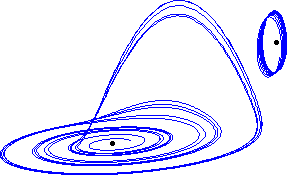
\includegraphics[width=0.26\textwidth]{RoessTrjs}%
~~(b)~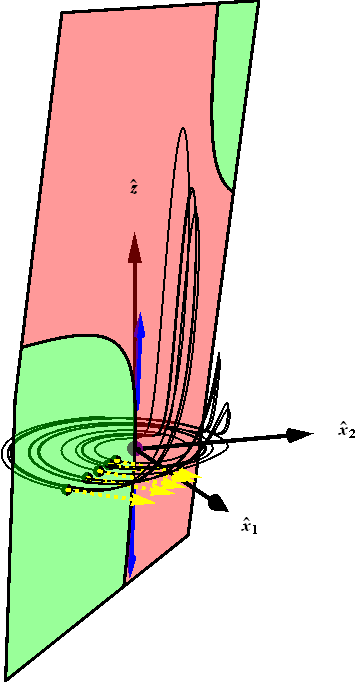
\includegraphics[width=0.18\textwidth,clip=true]{RoessNearEq2a}
    \caption{
(a)
R\"ossler \eqva\ and their invariant manifolds. The stable manifold of
the inner {\eqv} $\slicep{}^{(-)}$  is 1-dimensional and the unstable one
is a spiral-out focus. For the outer {\eqv} $\slicep{}^{(+)}$  the stable
manifold is a spiral-in focus (basin boundary for initial conditions that
either fall into the chaotic attractor, or escape to infinity) and the
unstable manifold is 1-dimensional.
(b)
\PoincSec\ plane through the inner {\eqv} $\slicep{}^{(-)}$ and
its stable eigenvector. The chart $\PoincS_{-}$ of the $\slicep{}^{(-)}$
neighborhood, bounded by its \poincBord, is highlighted by (light) green.
    }
\label{fig:RoessTrjs}
\end{figure}
%%%%%%%%%%%%%%%%%%%%%%%%%%%%%%%%%%%%%%%%%%%%%%%%%%%%%%%%%%%%%%%%%%%%%

%%%%%%%%%%%%%%%%%%%%%%%%%%%%%%%%%%%%%%%%%%%%%%%%%%%%%%%%%%%%%%%%%%%%%
% supercedes \label{fig:RoessBothEq}
\begin{figure}%[H]
\begin{center}
(a)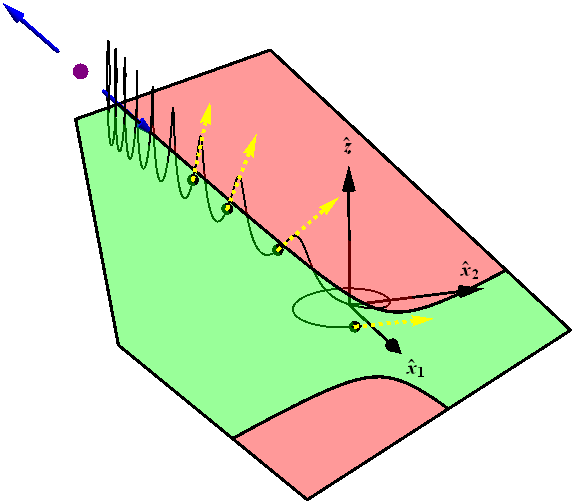
\includegraphics[width=0.23\textwidth,clip=true]{RoessFarEq2}%
(b)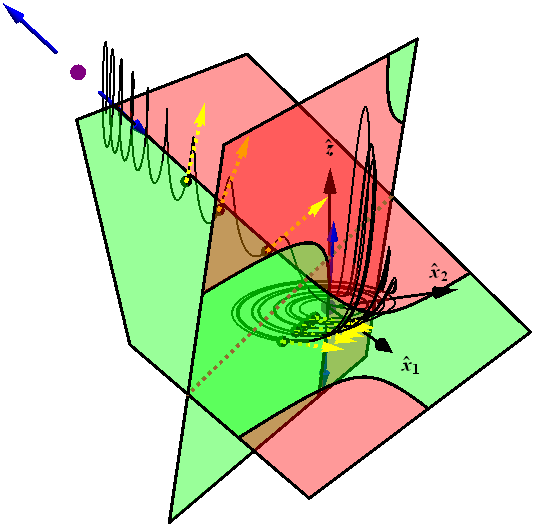
\includegraphics[width=0.23\textwidth,clip=true]{RoessSctAtlas2}
\end{center}
  \caption[R\"ossler section, outer {\eqv}]{
(a)
  A section through the outer {\eqv} $\slicep{}^{(+)}$  and its unstable
  eigenvector. The velocity $\vel(\sspRed_n)$ at the $n$th section is
  indicated by (yellow) vector.
(b)
  A two-chart atlas for R\"ossler flow, with the local sections of
  oriented and combined so that the ridge (intersection of the two
  sections, indicated by the dotted brown line) lies approximately
  between the \template s.
  } \label{fig:RoessFarEq}
\end{figure}
%%%%%%%%%%%%%%%%%%%%%%%%%%%%%%%%%%%%%%%%%%%%%%%%%%%%%%%%%%%%%%%%%%%%%

%%%%%%%%%%%%%%%%%%%%%%%%%%%%%%%%%%%%%%%%%%%%%%%%%%%%%%%%%%%%%%%%%%%%%
% DB 04-13-2012: At some point somebody put the R�ssler figures together
% but left this behind....
%\begin{figure}%[H]
%\begin{center}
%\end{center}
%  \caption{
%  } \label{fig:RoessBothEq}
%\end{figure}
%%%%%%%%%%%%%%%%%%%%%%%%%%%%%%%%%%%%%%%%%%%%%%%%%%%%%%%%%%%%%%%%%%%%%

%\subsection{R\"ossler two-chart atlas}

For R\"ossler flow, ${\cal S}$ condition \refeq{eq:sspRSing} yields a
quadratic condition in 3 dimensions, so \poincBord s\ drawn in
\reffig{fig:RoessTrjs}\,(b) and \reffig{fig:RoessFarEq} are conic sections. The two
charts meet at a ridge, and together do a pretty good job as the 2-chart
atlas of the interesting R\"ossler dynamics, \reffig{fig:RoessFarEq}. As
explained in ChaosBook.org\cite{DasBuch}, due to extreme contraction
rate, the section in \reffig{fig:RoessTrjs}\,(b) is for all practical
purposes 1\dmn, and the associated return map yields all \po s of the
3\dmn\ flow.

In 3 dimensions everything -sections, ridges, \poincBord s-  can be
drawn. But what about high-dimensional flows? The point is that while it
is impossible to visualize  $(d\!-\!2)$\dmn\ {\poincBord}, a point is a
point, and a line is a line in a projection from any number of
dimensions, so a trajectory crossing of both a section and a {\poincBord}
can be easily determined and visualized in any dimension.

To summarize: we can chart a region of \statesp\ of interest, by a
picking a sufficient number of \template s and the associated charts over
their neighborhoods, each bounded by \poincBord s and ridges.

Two concluding remarks on what sections \emph{are not}:

(1) A \PoincSec\ is {\em not} a projection onto a
lower-dimensional space: Rather, it is a local change of coordinates to a
direction along the flow $\vel(\sspRed)$, and the remaining coordinates
transverse to it. No information about the flow is lost; the full space
trajectory can always be reconstructed by integration from its point
$\sspRed$ in the section.

(2) The method of \PoincSec s is {\em not} equivalent to
\emph{strobing} a flow at a sequence of instants in time. While
`strobing' is what any numerical integrator does, by representing a
trajectory by a sequence of time-integration step separated points, this
is no reduction of a flow to a codimension 1 manifold, as the sequence of
strobed points still resides in the full \statesp\ $\pS$, of
dimensionality $d$.
